\documentclass[final,hyperref={pdfpagelabels=false}]{beamer}

\mode<presentation>{\usetheme{I6pd2_hugo}}
\usepackage[english]{babel}
\usepackage[utf8]{inputenc}
\usepackage{amsmath,amsthm, amssymb, latexsym, subfigure, graphicx,array,booktabs,tabularx}
%\usepackage{times}\usefonttheme{professionalfonts}  % obsolete
%\usefonttheme[onlymath]{serif}
\boldmath
\usepackage[orientation=portrait,size=a0,scale=1.4,debug]{beamerposter}
% change list indention level
% \setdefaultleftmargin{3em}{}{}{}{}{}
\usecaptiontemplate{
\small
\structure{\insertcaptionname~\insertcaptionnumber:}
\insertcaption
}


%\usepackage{snapshot} % will write a .dep file with all dependencies, allows for easy bundling

\newcolumntype{Z}{>{\centering\arraybackslash}X} % centered tabularx columns
\newcommand{\pphantom}{\textcolor{ta3aluminium}} % phantom introduces a vertical space in p formatted table columns??!!

\listfiles

%%%%%%%%%%%%%%%%%%%%%%%%%%%%%%%%%%%%%%%%%%%%%%%%%%%%%%%%%%%%%%%%%%%%%%%%%%%%%%%%%%%%%%
 
\title{{BEAM COUPLING IMPEDANCE OF THE NEW BEAM SCREEN OF THE LHC INJECTION KICKER MAGNETS}
\author{H. Day, M.J. Barnes, F. Caspers, E. Métral, B. Salvant, J. Uythoven}
\institute[CERN]{CERN, Geneva, Switzerland}
\date[June 2014]{June 2014}

%%%%%%%%%%%%%%%%%%%%%%%%%%%%%%%%%%%%%%%%%%%%%%%%%%%%%%%%%%%%%%%%%%%%%%%%%%%%%%%%%%%%%%
\newlength{\columnheight}
\setlength{\columnheight}{105cm}


%%%%%%%%%%%%%%%%%%%%%%%%%%%%%%%%%%%%%%%%%%%%%%%%%%%%%%%%%%%%%%%%%%%%%%%%%%%%%%%%%%%%%%
\begin{document}
\begin{frame}
  \begin{columns}
    % ---------------------------------------------------------%
    % Set up a column 
    \begin{column}{.49\textwidth}
      \begin{beamercolorbox}[center,wd=\textwidth]{postercolumn}
        \begin{minipage}[T]{.95\textwidth}  % tweaks the width, makes a new \textwidth
          \parbox[t][\columnheight]{\textwidth}{ % must be some better way to set the the height, width and textwidth simultaneously
            % Since all columns are the same length, it is all nice and tidy.  You have to get the height empirically
            % ---------------------------------------------------------%
            % fill each column with content            
            \begin{block}{Abstract}
\small{
The LHC injection kicker magnets experienced significant beam induced heating of the ferrite yoke, with high beam currents circulating for many hours, during operation of the LHC in 2011 and 2012. The causes of this beam coupling impedance were studied in depth and an improved beam screen implemented to reduce the impedance. Results of measurements and simulations of the new beam screen design are presented in this paper: these are used to predict power loss for operation after long shutdown 1 and for proposed HL-LHC operational parameters.
}
\end{block}
            \vfill

	\begin{block}{Introduction}
\small{
\begin{figure}
\subfigure[]{
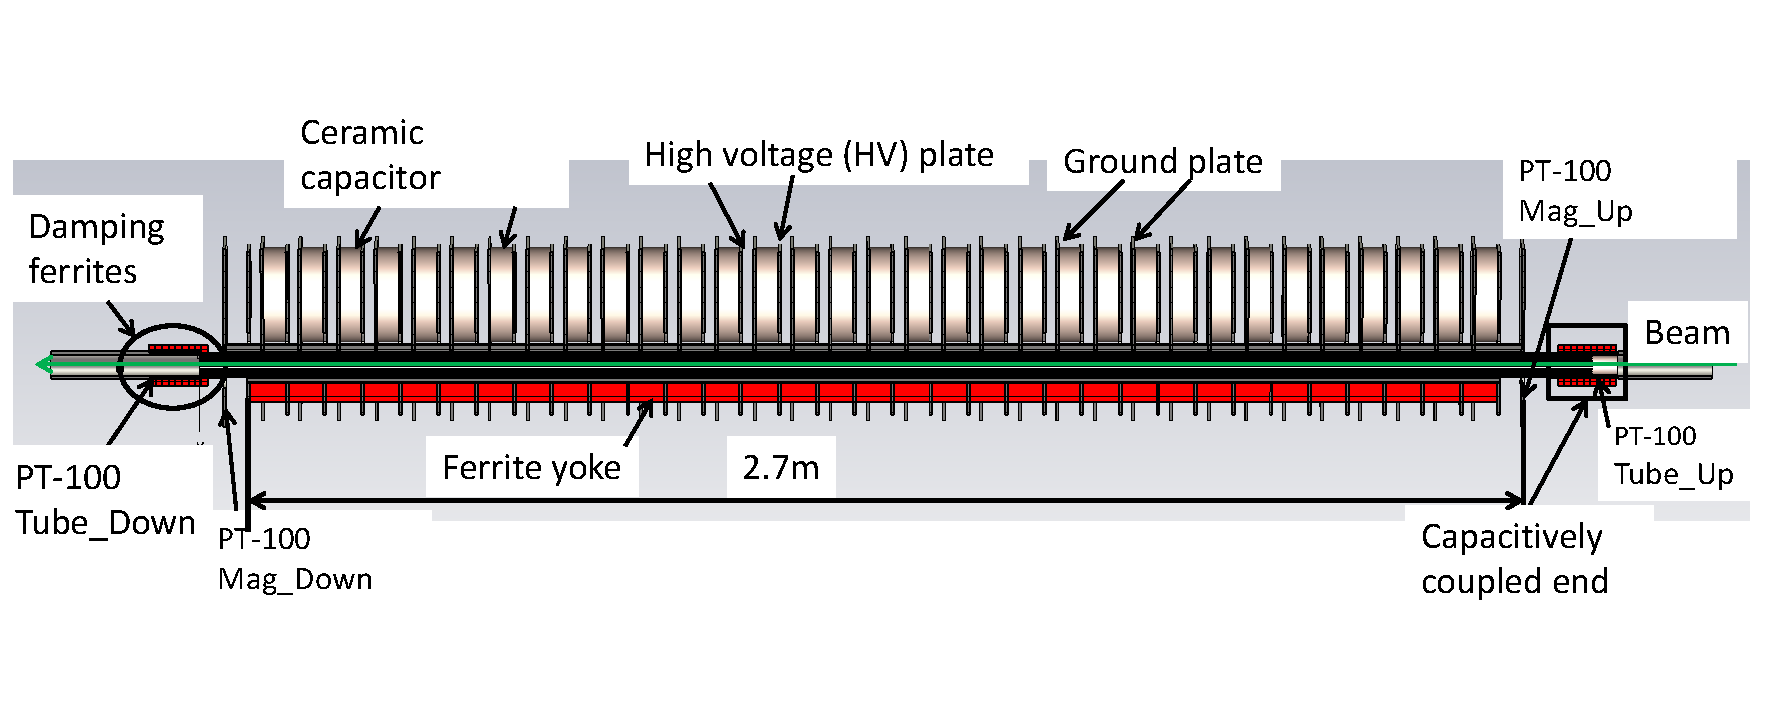
\includegraphics[width=0.5\textwidth]{figures/MKICrossSectionYZ.pdf}
\label{fig:mkiStruct}
}
\subfigure[]{
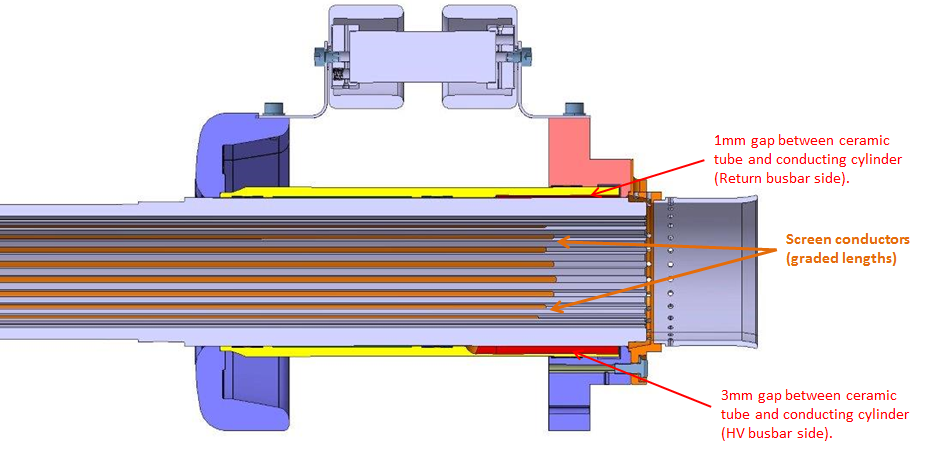
\includegraphics[width=0.45\textwidth]{figures/screenDesignCrossSection.png}
\label{fig:SideView}
}
\caption{\subref{fig:mkiStruct} The structure of the MKI and \subref{fig:SideView} the internal structure of the beam screen.}

\end{figure}

	\begin{itemize}
	\item{During operation of the LHC in 2011 and 2012, high temperatures were observed in the LHC injection kicker magnets (MKIs), becoming higher as the bunch intensity was increased to reach higher luminosities [1].}
	\item{The heating was determined to be caused by beam-induced heating due to the circulating beam interacting with the real component of the longitudinal beam coupling impedance in the magnet. The hottest magnet before technical stop 3 (TS3), MKI8D, was replaced with a new beam screen in TS3 to improve the screening of the ferrite yoke (structure shown in Fig.~\ref{fig:mkiStruct}).}
	\item{The improved screening was shown to be highly effective, strongly reducing the temperature of MKI8D, seen in Fig.~\ref{fig:HeatingPt8}, where it can be seen MKI8D changes from being the hottest magnet at IP8 to the coldest after TS3 [2].}

	\end{itemize}
\begin{figure}
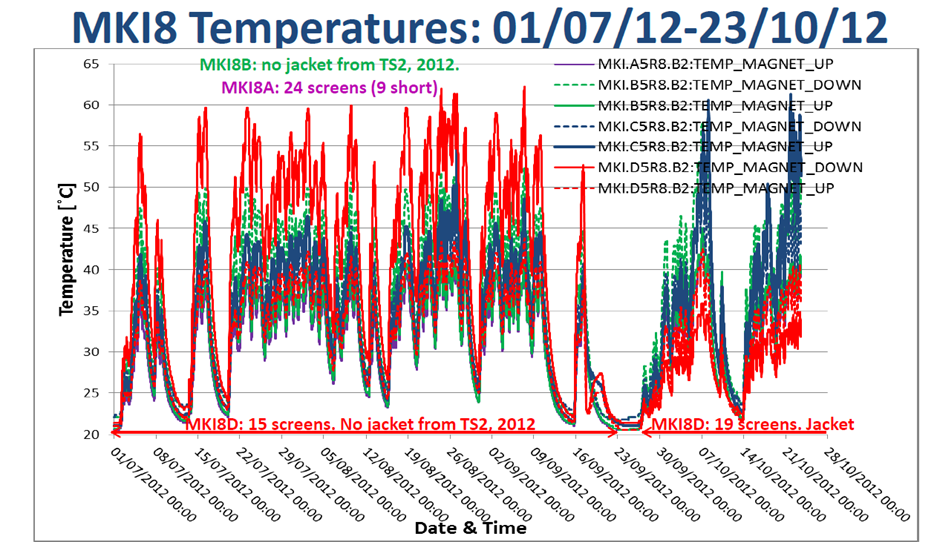
\includegraphics[width=0.5\textwidth]{figures/mki8-temps-post-ts3.png}
\caption{Heating of the MKIs at IP8 before and after TS3.}
\label{fig:HeatingPt8}
\end{figure}
}
	\end{block}
 \vfill
\begin{block}{New Beam Screen Design}
\small{
\begin{itemize}
\item{A new screen design has been proposed [3] for installation in the MKIs during long shutdown 1 (LS1) which aims to include 24 screen conductors in the design, whilst lowering the surface electric field on the ceramic tube during kicker pulsing, shown in Fig.~\ref{fig:SideView}.}




\item{The capacitively coupled end is significantly changed:}
\begin{itemize}
\item{The external metallization is replaced by an external metal tube which steps away from the ceramic tube near the ends of the screen conductors. This reduces the surface electric field on the ceramic tube significantly. Tapering the length of the conductors also helps this reduction.}
\item{This reduction allows 24 screen conductors to be placed back in the beam screen, greatly improving the screening of the ferrite yoke from the beam.}
\end{itemize}
\item{In addition the thermal emissivity of the inside of the vacuum tank is planned to be increased to help improve heat evacuation from the tank.}
\end{itemize}
}
\end{block}
            \vfill

\vfill
\begin{block}{References}
\begin{enumerate}
\item{\small{E. Métral \emph{et al}., \emph{Beam-Induced Heating/Bunch Length/RF and Lessons for 2012}, LHC Performance Workshop, Chamonix 2012, CERN-ATS-2012-069}}
\item{\small{M.J. Barnes \emph{et al}., \emph{Beam Induced Ferrite Heating of the LHC Injection Kickers and Proposals for Improved Cooling}, IPAC2013, MOPWA031}}
\item{\small{M.J. Barnes \emph{et al}., \emph{Upgrade of the LHC Injection Kicker Magnets}, IPAC2013, MOPWA030}}
\item{\small{T. Kroyer, F. Caspers, and E. Gaxiola, \emph{Longitudinal and Transverse Wire Measurements for the Evaluation of Impedance Reduction Measures on the MKE Extraction Kickers} CERN, Geneva, CERN-AB-Note-2007-028, Jul 2007}}
\item{\small{Hugo Day, PhD Thesis, June 2013}}
\end{enumerate}
\end{block}
         \vfill
          }
        \end{minipage}
      \end{beamercolorbox}
    \end{column}
    % ---------------------------------------------------------%
    % end the column

    % ---------------------------------------------------------%
    % Set up a column 
    \begin{column}{.49\textwidth}
      \begin{beamercolorbox}[center,wd=\textwidth]{postercolumn}
        \begin{minipage}[T]{.95\textwidth} % tweaks the width, makes a new \textwidth
          \parbox[t][\columnheight]{\textwidth}{ % must be some better way to set the the height, width and textwidth simultaneously
            % Since all columns are the same length, it is all nice and tidy.  You have to get the height empirically
            % ---------------------------------------------------------%
            % fill each column with content
\begin{block}{Impedance Measurements of New Design}
\begin{itemize}
\item{The beam coupling impedance for all MKIs with the new beam screen design is measured before bake out and HV conditioning to ensure consistency between magnets and to foresee any possible problems with regards to heating}
\item{Measurements is typically done using the coaxial resonant method due to it's sensivity to low impedances. Additional measurements with the classical coaxial method are done as time allows}
\end{itemize}
\begin{figure}
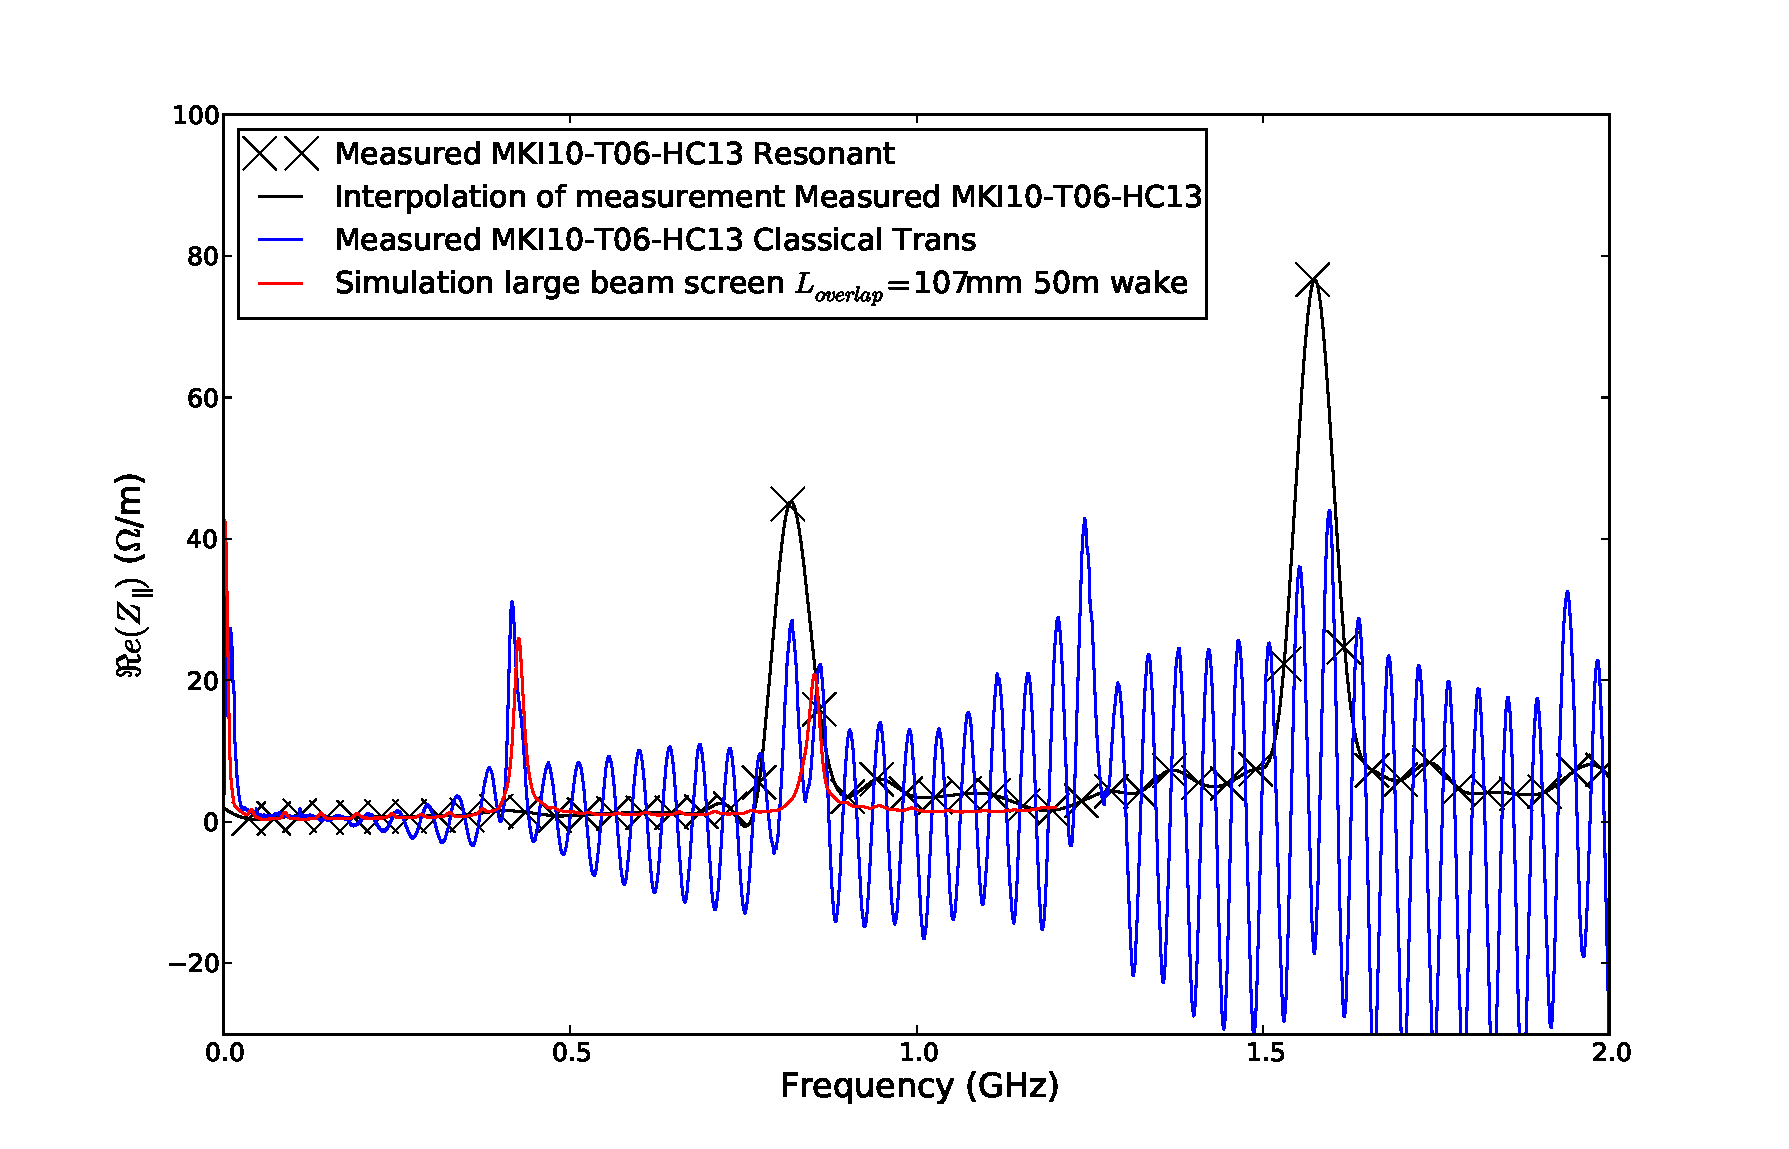
\includegraphics[width=0.5\textwidth]{figures/compTransmissionResSimulations.pdf}
\caption{\small{Impedance measurements of one MKI using the resonant coaxial wire method and the classical coaxial method, with comparisons to impedance simulations of the new design.}}
\end{figure}
\begin{table}
\label{tab:beamPar}
\caption{Beam parameters for power loss calculations}
\begin{center}
\begin{tabular}{c | c | c | c | c}
\small{Running Mode} & $N_{b}$ $10^{11}$ & $n_{bunches}$ & bunch length (ns) & Bunch separation (ns) \\ \hline 
\small{Pre-LS1} & 1.6 & 1380 & 1.2 & 50ns \\ \hline
\small{Post-LS1} & 1.15 & 2808 & 1.0 & 25ns \\ \hline
\small{HL-LHC 25ns}& 2.2 & 1380 & 1.0 & 25ns \\ \hline
\small{HL-LHC 50ns}& 3.5 & 2808 & 1.0 & 50ns \\
\end{tabular}
\end{center}
\end{table}

\begin{table}
\label{tab:heating-mki-screen-designs}
\caption{\small{The power loss expected  in the MKIs for the magnets measured so far. All power losses are given in W/m.}}
\begin{center}
\begin{tabular}{c | c | c | c | c}
\small{Screen Design} & \small{Pre-LS1} & \small{Post-LS1} & \small{HL-LHC 50ns} & \small{HL-LHC 25ns} \\ \hline 
\small{New Design} & 21-35 & 34-52 & 151-240 & 125-191 \\ \hline
\small{15 screen conductors} & 68 & 117 & 538 & 432 \\ \hline
\small{Old MKI8D (twisted)} & 168 & N/A & N/A & N/A \\ \hline
\small{19 screen conductors} & 52 & 76 & N/A & N/A \\
\end{tabular}
\end{center}
\end{table}

\end{block}
\vfill
\begin{block}{Resonant Coaxial Impedance Measurements}
\begin{itemize}
\item{The resonant coaxial impedance measurement method turns the device under test (DUT) in a coaxial resonator by running a coaxial line through the device and weakly capacitively coupling the device to the VNA circuit.}
\item{Measurement of the Q factor of this resonance very accurate measurement of the losses of the system can be made and the impedance measured.} 
\item{Drawbacks are that resonant frequencies are dependant on the length of the DUT meaning frequency resolution can be poor for short devices.}
\end{itemize}
\begin{equation}
f_{0} = \frac{nc}{2L}
\end{equation}
\begin{figure}
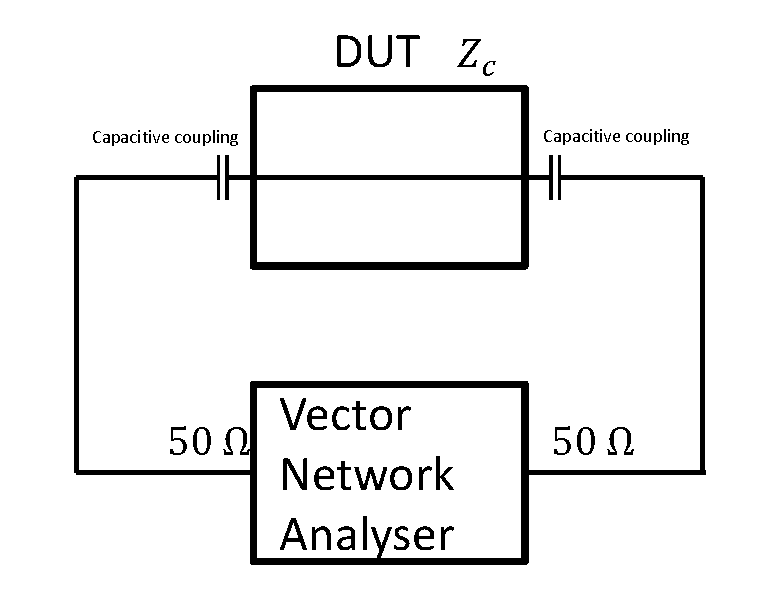
\includegraphics[width=0.25\textwidth]{figures/wire_meas_single_wire.pdf}
\caption{Schema of the measurement setup for the coaxial resonant wire method.}
\label{fig:measResonantMethod}
\end{figure}
\begin{itemize}
\item{Length can be increased by artificially lengthening the structure - the use of low loss coaxial cables being a solution (their losses are well characterised and the length known). Other solutions may be possible also (inductances or capacitances to increase the electrical length) however these would make measurements of the imaginary impedance of the device complicated.}
\item{More details of the analysis technique can be found in [4] and [5]}
\end{itemize}
\begin{figure}
\subfigure[]{
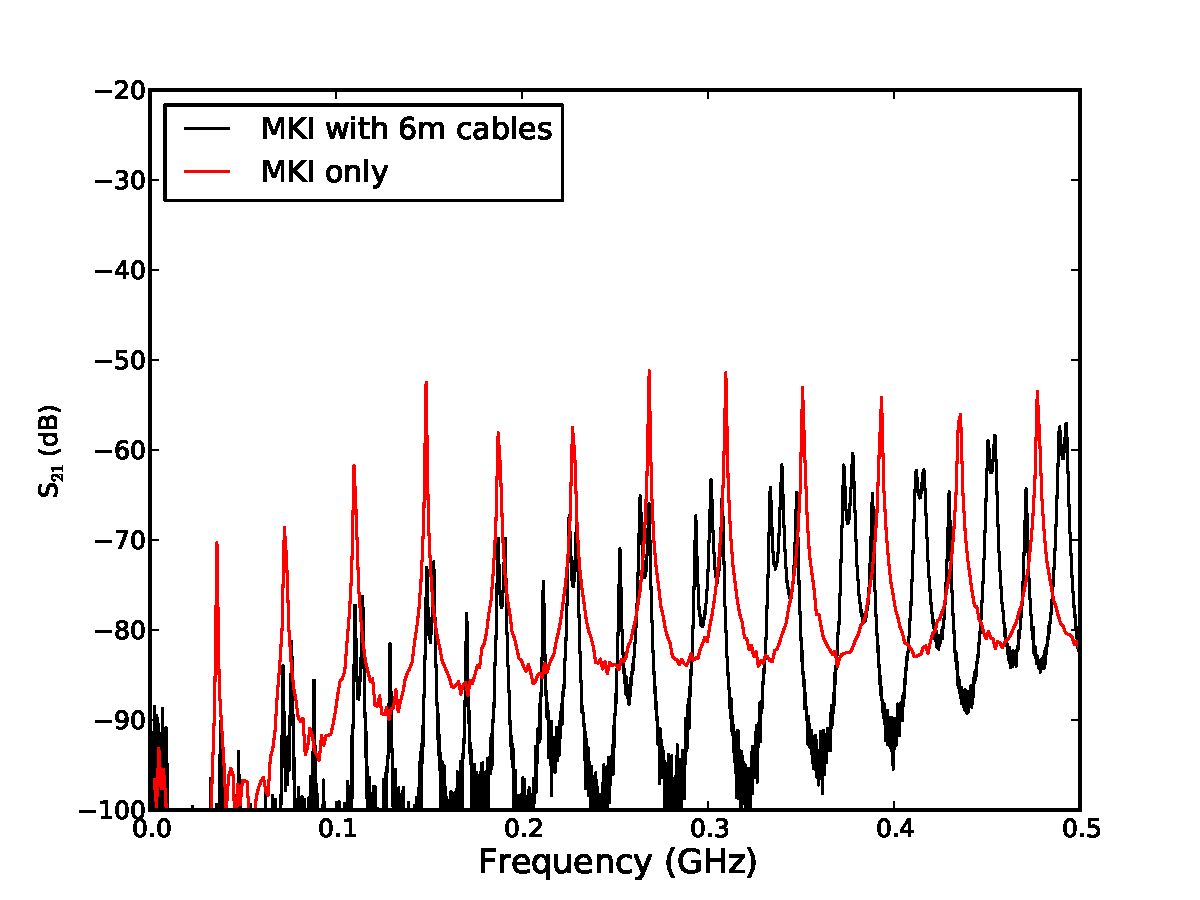
\includegraphics[width=0.4\textwidth]{figures/resMethodPlotsS21.pdf}
\label{fig:s21Res}
}
\subfigure[]{
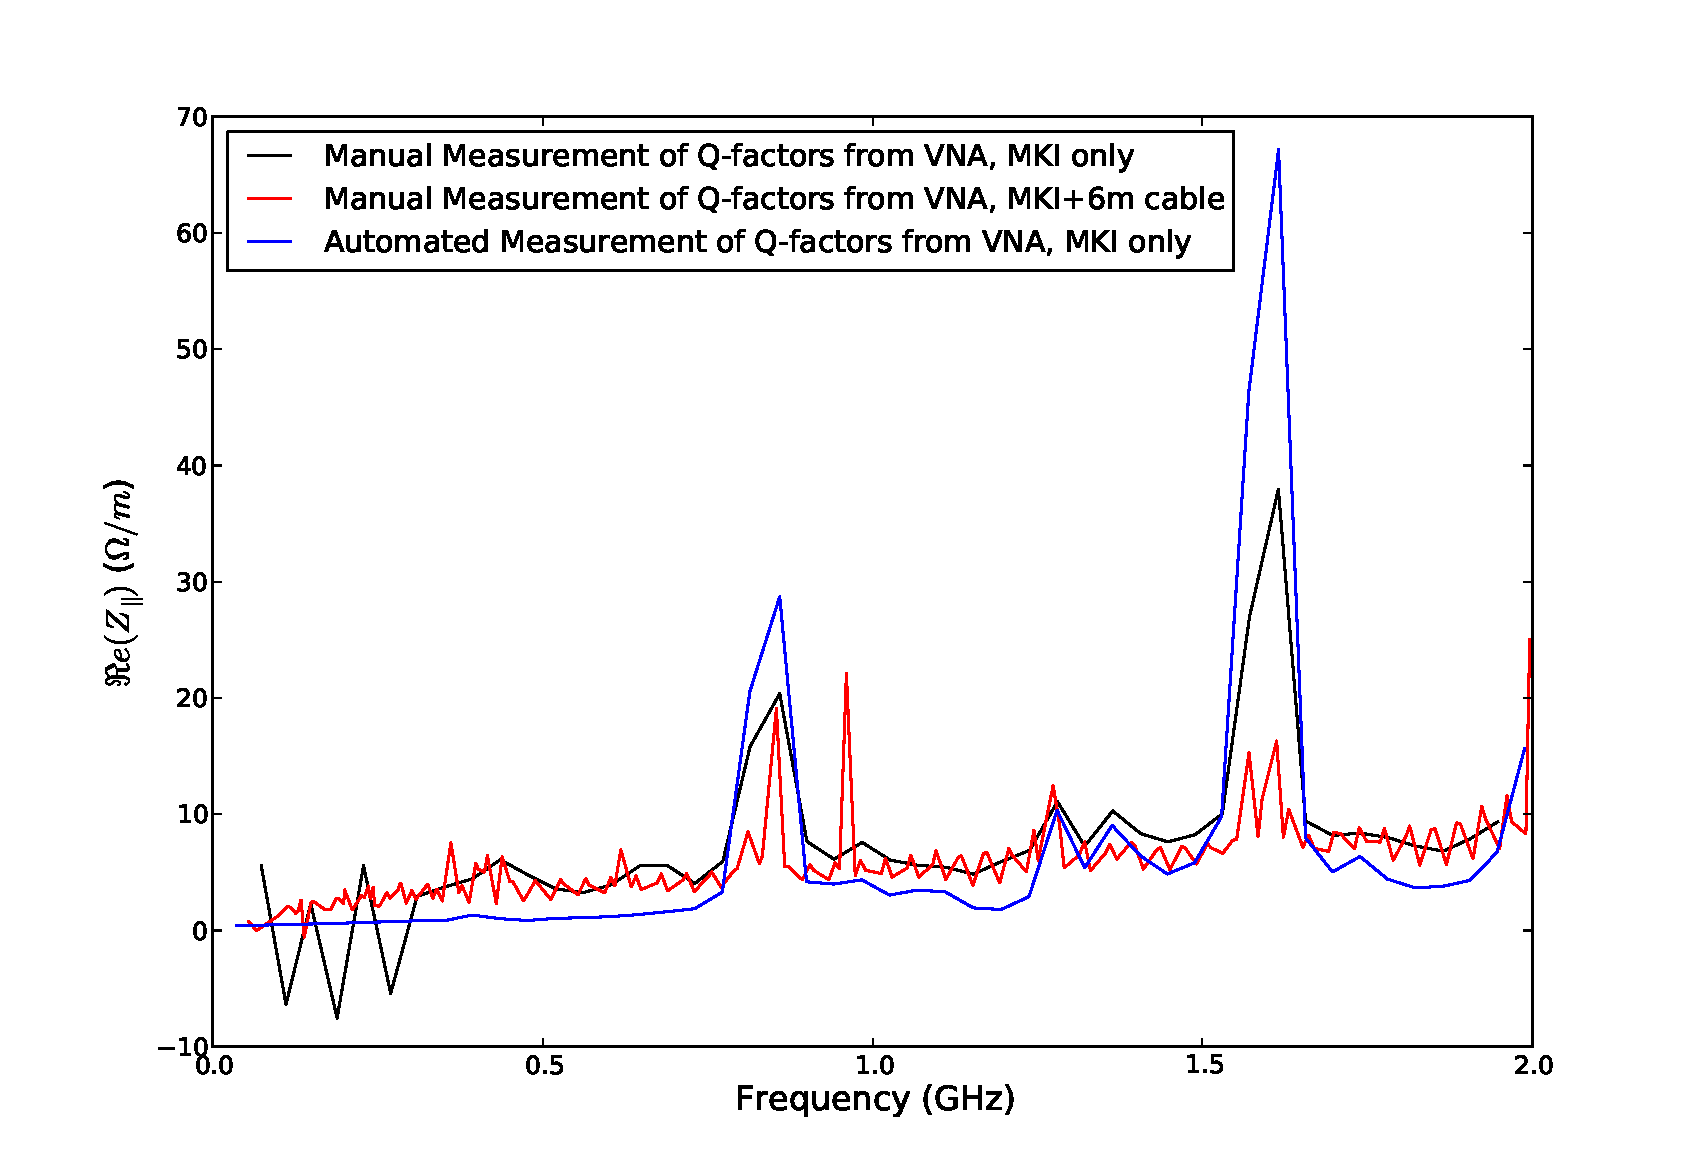
\includegraphics[width=0.45\textwidth]{figures/resMethodPlotsImp.pdf}
\label{fig:resImp}
}
\caption{\subref{fig:s21Res} $S_{21}$ and \subref{fig:resImp} impedance measurements of a number of configurations for measurement setups for an MKI with the new screen design.}
\end{figure}
\end{block}

%
%\begin{block}{Beam Coupling Impedance of the New Screen Design}
%\small{
%\begin{itemize}
%\item{8 magnets with the new screen design have been produced to date, all measured using the resonant coaxial wire method}
%\item{The longitudinal impedance is simulated for 3 cases; the beam screen before TS3 for all MKIs, the screen for the revised MKI8D installed during TS3, and the proposed screen design for post LS1. The real components of all are shown in Fig.~\ref{fig:MKIScreenImp}}
%
%\end{itemize}
%
%\begin{figure}
%\subfigure[]{
%\includegraphics[width=0.4\textwidth]{realImp.pdf}
%\label{fig:MKIScreenImp}
%}
%\subfigure[]{
%\includegraphics[width=0.4\textwidth]{mki-overlap-len-real-imp-zoom.pdf}
%\label{fig:mkiOverlapRes}
%}
%\caption{\subref{fig:MKIScreenImp} The real component of the longitudinal beam coupling impedance of the existing MKIs, the replacement MKI8D and the proposed beam screen design for after LS1. \subref{fig:mkiOverlapRes} The resonant frequency due to different lengths of the overlap of the screen conductors with external metallization from simulations and calculated from \ref{eqn:imp-overlap-fres}, are shown as blue vertical lines.}
%\end{figure}
%
%\begin{itemize}
%\item{For the well screened magnet (the ferrite yoke is not visible to the circulating beam), the impedance is dominated by a resonance due to the overlapping area between the screen conductors and the external metallization/metal tube. The resonant frequency $f_{res}$ is given by}
%
%\begin{equation}
%\small{f_{res} = \frac{nc}{\sqrt{\epsilon_{r}}2 \left( L_{overlap} + \delta_{fringe} \right)},}
%\label{eqn:imp-overlap-fres}
%\end{equation}
%
%\item{where $\epsilon_{r}$ is the relative permittivity of the surrounding medium (in this case $\epsilon_{r} \approx 10$ for the alumina ceramic tube), $c$ is the speed of light, $L_{overlap}$ is the length of the overlap, and $\delta_{fringe}$ is a factor to take into account fringe fields, which depends on the distance between the screen conductors and the external metallization/metal tube.}
%\item{Examples of the predicted impedance for different lengths of overlap between 80 mm and 120 mm are shown in Fig.~\ref{fig:mkiOverlapRes} compared to simulated impedance. These show very good agreement between the two.}
%\end{itemize}
%
%
%}

\vfill

          }
          % ---------------------------------------------------------%
          % end the column
        \end{minipage}
      \end{beamercolorbox}
    \end{column}
    % ---------------------------------------------------------%
    % end the column
  \end{columns}

  %\tiny\hfill\textcolor{ta2gray}{Created with \LaTeX \texttt{beamerposter}  \url{http://www-i6.informatik.rwth-aachen.de/~dreuw/latexbeamerposter.php}}
%  \tiny\hfill{Created with \LaTeX \texttt{beamerposter}  \url{http://www-i6.informatik.rwth-aachen.de/~dreuw/latexbeamerposter.php} \hskip1em}
\end{frame}
\end{document}


%%%%%%%%%%%%%%%%%%%%%%%%%%%%%%%%%%%%%%%%%%%%%%%%%%%%%%%%%%%%%%%%%%%%%%%%%%%%%%%%%%%%%%%%%%%%%%%%%%%%
%%% Local Variables: 
%%% mode: latex
%%% TeX-PDF-mode: t
%%% End:
